\section{Anforderungen}
\begin{itemize}
	\item Wenigstens ein Objekt in der Szene sollte bewegte Gliedmaßen haben.
	\item Wenigstens eine Szene sollte die Kameraeinstellung variieren, z.B. in die Szene hineinfahren, schwenken oder zoomen.
	\item Setzen Sie ein verarbeitetes Bild ein, z.B. als Höhenprofil, Kulisse oder Textur.
	\item Erstellen sie einen animierten Titel.
	\item Setzen Sie Überblendungen ein, um den Schnitt zwischen zwei Kamerapositionen oder anderen Bildwechseln zu betonen oder zu kaschieren.
	\item Setzen Sie Sound-Effekte zum Vertonen ein.
\end{itemize}
%
\section{Handlung}
Wir setzen ein Squashspiel mit schwebenden Squashschlägern ohne Spieler in PovRay um. Zwei Zuschauer kommen aus einem Eingang in die Halle und setzen sich auf die Tribüne vorm Squash Court. Die Kamera fliegt durch die Courttür in den Court. Die Tür schließt sich und das Spiel beginnt. Nach ein paar Ballwechseln ist das Spiel vorbei und die Kamera zeigt die jubelnden Zuschauer. 
%
\section{Technisches}
\subsection{Grundlegendes und Konventionen}
\begin{itemize}
	\item Eine PovRay Distanzeinheit von $1.0$ entspricht $1.0$ Meter in der Realität
	\item Eine PovRay Clockeinheit von $1.0$ entspricht $1.0$ Sekunden in der Realität
	\item Das PovRay Koordinatensystem hat seinen Ursprung in der linken unteren hinteren Ecke des Squash Courts (siehe Grafik~\ref{fig:squashcourt} und \ref{fig:halloutline}).
\end{itemize}
%
\begin{figure}%[h!]
	\centering
	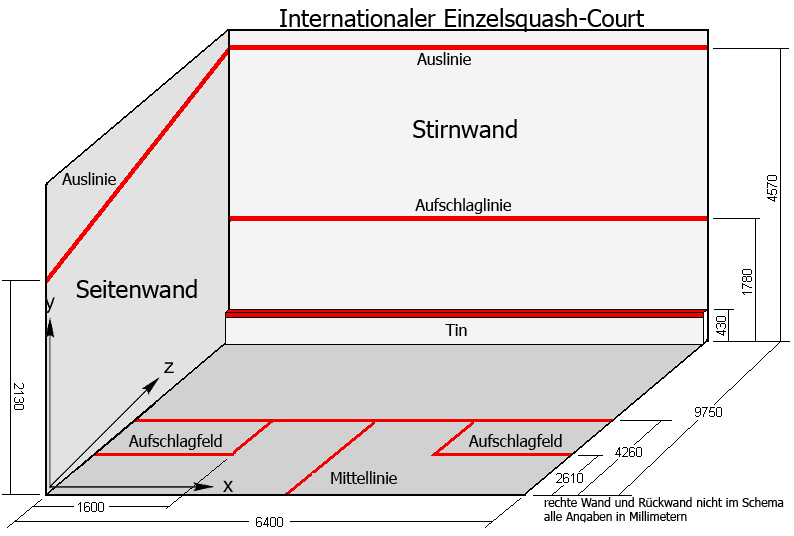
\includegraphics[width=.9\linewidth]{images/Squash_Court.png}
	\caption{Maße eines Squash Courts + PovRay Koordinatensystem}\label{fig:squashcourt}
\end{figure}
\begin{figure}%[h!]
	\centering
	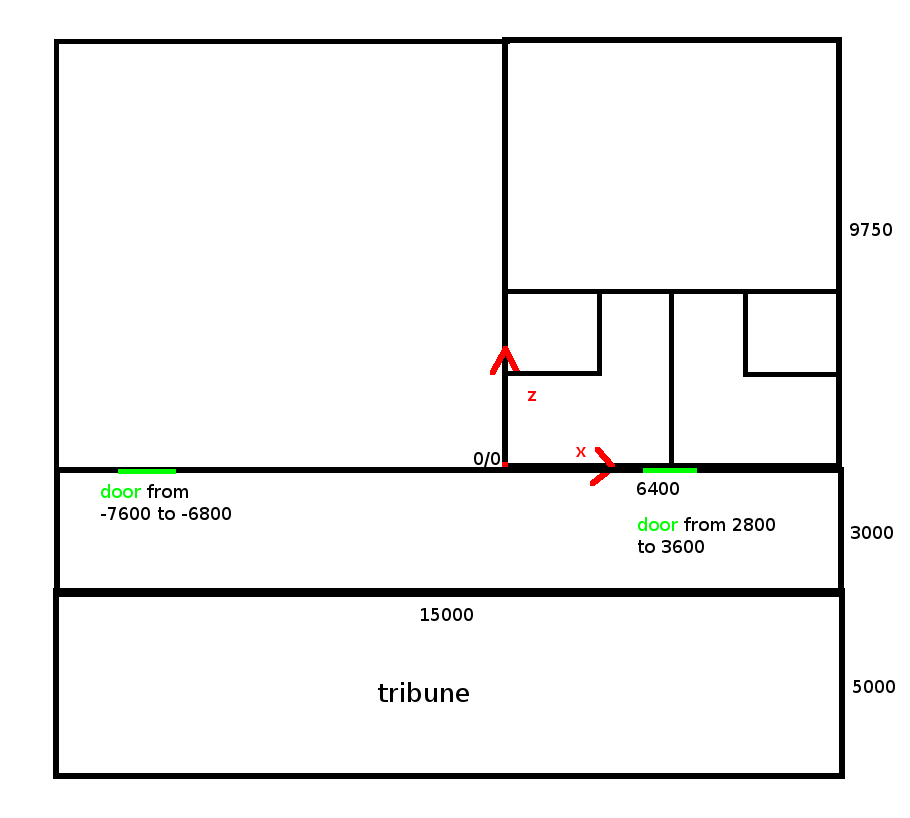
\includegraphics[width=.7\linewidth]{images/hall_outline.png}
	\caption{Grundriss der gesamten Karte}\label{fig:halloutline}
\end{figure}
\subsection{Aufbau des Programms}
\subsubsection{Organisation der Dateien}
Jede Szene hat eine eigene \texttt{pov} und \texttt{ini} Datei, die alle den Präfix \texttt{animation} tragen. So kann jede Szene ihre eigenen Einstellungen haben und einzeln gerendered werden. Alle statischen Programmteile, wie die komplette Halle, aber auch das Modell der Zuschauer, des Balles sowie der Schläger befinden sich in einem Unterverzeichnis names \texttt{static}. Jede Szene inkludiert die statischen Parts. Dabei muss nur die Datei \texttt{main\_static.inc}, sowie \texttt{figure.inc} inkludiert werden, die alle weiteren Parts enthalten (siehe Grafik~\ref{fig:aufbau}).
\begin{figure}[h!]
	\centering
	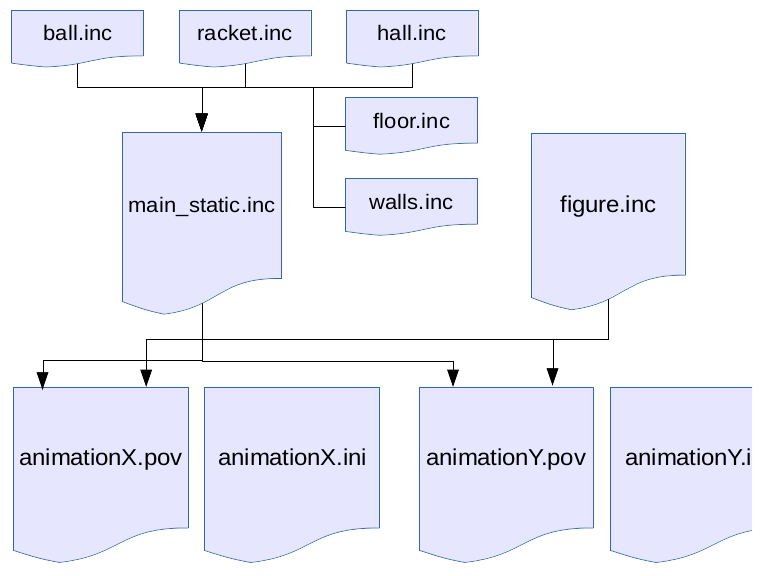
\includegraphics[width=.9\linewidth]{images/aufbau_grafisch.png}
	\caption{Organisation der Dateien}\label{fig:aufbau}
\end{figure}

\subsubsection{Schematischer Aufbau einer \texttt{animationX.pov} Datei}
Die PovRay Clock läuft hier nicht, wie zumeist, von $0.0$ bis $1.0$ pro Szene, sondern entspricht Sekunden in der Realität. Da wir ein Squashspiel erstellen, ist es von Vorteil, in Sekunden zu rechnen, weil so Animation sowie die Ballgeschwindigkeit realistischer dargestellt werden können. 

Um bei Animationen dennoch eine Zahl zwischen $0.0$ und $1.0$ zu erhalten, wird die Clock in jedem Abschnitt skaliert. Damit bleiben die Vorteile der normalisierten Zeit, nämlich dass Animationen übertragbar sind, sowie leichtere Rechnungen bei der Erstellung der Animationen, erhalten.

Der folgende Quellcode zeigt zusammenfassend die Struktur der Szenen:\\

\begin{lstlisting}[caption=Schematischer Aufbau einer animationX.pov Datei]
#include ...

#switch(clock)
	#range (timeA, timeB)
		#local clk = (clock - timeA) / (timeB - timeA);
		// time dependend animation code like rackets and ball comes
		// here using the locally defined clk variable
	#break
	#range (timeB, timeC)
		#local clk = (clock - timeB) / (timeC - timeB);
		// time dependend animation code like rackets and ball comes
		// here using the locally defined clk variable
	#break
#end
\end{lstlisting}
\vspace{1.5em}
Zunächst kommen die notwendigen includes, anschließlichen wird ein \texttt{switch} Statement auf die globale \texttt{clock} Variable aufgerufen. PovRay erlaubt im \texttt{switch} ein \texttt{range} Statement zu benutzen, sodass man Zeitspannen festlegen kann. In jeder dieser Zeitspannen wird die lokale Variable \texttt{clk} definiert, die die normalisierte Zeit zwischen $0.0$ und $1.0$ enthält. So können einfach Animation definiert werden. Falls eine Animation zu langsam ist, kann die Zeitspanne einfach verkürzt werden und die Animation läuft schneller ab.

\subsubsection{Die Flugbahn des Balles}
Um die Flugbahn des Balles einigermaßen realistisch zu gestalten, wurden die Gleichungen für den schiefen Wurf verwendet. Allerdings wurde aus Gründen der Einfachheit die Reibung nicht berücksichtigt. Ebenso wurde die Abbremsung des Balles an einer Wand oder am Boden lediglich geschätzt.

Die Berechnung der Flugbahn wurde in ein Makro ausgelagert, welches in\\ \texttt{ball\_trajectory.inc} zu finden ist. Im Laufe der Entwicklung haben wir Mängel festgestellt, sodass auch \texttt{ball\_trajectory2.inc} und \texttt{ball\_trajectory3.inc} entstanden sind. 

Version2 behebt den Fehler, dass die Richtung des Balles in dem vertikalen Abschlagwinkel durch das Vorzeichen enthalten ist. Dies führt dazu, dass es in Richtung der Wand keine negativen vertikalen Winkel und in Richtung der Glasscheibe keine positiven vertikalen Winkel geben kann. Also wurde die Richtung des Balles in ein extra Parameter ausgelagert.

Weil PovRay sich keine Zustände zwischen dem Generieren von zwei Bildern merken kann, wird für jedes Bild die Flugbahn neuberechnet. Da erschien es am einfachsten, wenn der Ball eine Wand oder den Boden berührt, ab dort eine neue Flugbahnberechnung einzuleiten, indem das Makro erneut mit angepasstem Winkel und Geschwindigkeit aufgerufen wird. Problematisch an dieser Variante ist, dass das Momentum des Ball in Richtung Boden (durch die Erdanziehung), welches ab dem Schlag des Balles immer größer wird, zurück auf $0$ gesetzt wird. Dies sorgt für unrealistische Flugbahnen. Version 3 des Makros behebt dies, indem der ursprüngliche Zeitpunkt des Schlages mit angegeben werden kann, woraus die momentane Geschwindigkeit Richtung Boden errechnet wird. Mit dieser Version sind recht realistische Ballwechsel möglich. Das folgende Listing zeigt den Quellcode der 3. Version:\\

\begin{lstlisting}[caption=Makro zur Generierung einer Flugbahn des Balles (verkürzt)]
#macro ball_trajectory3(p_start, v_start, vert_angle, hori_angle, ball_direction, local_clock, old_clock, old_v, old_y)
	#local x_val =  v_start*local_clock*sin(radians(hori_angle)) + p_start.x;
	#local y_val = old_v*old_clock*sin(radians(vert_angle)) - g/2 * pow(old_clock,2) + old_y;

	#if (ball_direction < 0)
		#local z_val = -v_start*local_clock*cos(radians(vert_angle)) + p_start.z;
	#else 
		#local z_val = v_start*local_clock*cos(radians(vert_angle)) + p_start.z;
	#end

	object {
		ball
		translate <x_val, y_val, z_val>
	}
#end
\end{lstlisting}
Die Parameter bedeuten folgendes:
\begin{itemize}
	\item \texttt{p\_start}: Die Startposition des Balles (Mittelpunkt des Balles) als 3D-Vektor
	\item \texttt{v\_vstart}: Die Geschwindigkeit des Balles
	\item \texttt{vert\_angle}: Der vertikale Abschlagwinkel des Balles. Ein Winkel von 0 führt dazu, dass der Ball parallel zum Boden fliegt. Bei einem positiven Winkel fliegt der Ball nach oben, bei einem negativen nach unten.
	\item \texttt{hori\_angle}: Der horizontale Abschlagwinkel des Balles. Ein Winkel von 0 führt dazu, dass der Ball parallel zu den Seitenwänden fliegen. Bei einem positiven Winkel fligen der Ball nach rechts, bei einem negativen nach links.
	\item \texttt{ball\_direction}: Die Flugrichtung des Balles. Bei $1$ fliegt der Ball Richtung Wand, bei $-1$ fliegt der Ball Richtung Glasscheibe.
	\item \texttt{local\_clock}: Zur Berechnung der Flugbahn wird die momentane Zeit benötigt. Wichtig ist, dass die Zeit nicht normalisiert sein darf, weil die Geschwindigkeit auch nicht normalisiert ist und in $m/s$ angegeben wird. Dennoch muss die Zeit zum Zeitpunkt des Schlages $0.0$ betragen. Deshalb wird grundsätzlich der Wert $clock - timeHit$ übergeben, also die unnormalisierte, in Sekunden laufende, Uhr abzüglich des Schlagzeitpunktes.
	\item \texttt{old\_clock}: Dieser Wert existiert erst ab v3 des Makros. Falls der Ball von einer Wand abprallt, ist \texttt{local\_clock} der Zeitpunkt des Abpralls.\texttt{old\_clock} kriegt dann den Wert des Abschlages (also $clock - timeHit$), damit darauf die aktuelle Geschwindigkeit in Richtung Boden berechnet werden kann. 
	\item \texttt{old\_v}: Dieser Wert existiert erst ab v3 des Makros. Bei einem Abprall von der Wand, verringert sich die Geschwindigkeit des Balles. Für die Berechnung der Geschwindigkeit Richtung Boden wird aber der alte Wert benötigt.
	\item \texttt{old\_y}: Dieser Wert existiert erst ab v3 des Makros. Enthält die Höhe des Balles zum Zeitpunkt des Abschlages, weil darauf die aktuelle Höhe auf Basis der Wurfparabel berechnet wird.
\end{itemize}

Das Makro berechnet den momentanen $x$, $y$ und $z$ Wert des Balles und verschiebt den Ball anschließend an diesen Punkt. 

\texttt{x\_val} ist der momentane $x$ Wert und hängt von der initialen Position (\texttt{p\_start.x}), der Geschwindigkeit, des Sinus' des horizontalen Winkels sowie von der aktuellen Zeit ab (siehe Zeile 2).

Der $y$ Wert \texttt{y\_val} hängt von nur den initialen Werten beim Abschlag ab, egal wie oft der Ball eine Wand berührt außer der vertikale Winkel. Der ändert sich bei einem Zusammenstoß mit einer Wand nach dem Prinzip Einfallswinkel=Ausfallswinkel. Die Schwerkraft ist hier mit $g$ benannt und wird woanders global im Code definiert. Mit $g$ sowie der Geschwindigkeit, dem vertikalen Winkel, der ursprünglichen Höhe, soie der Zeit ab dem Schlag kann die momentane Höhe bestimmt werden.

Der $z$ Wert \texttt{z\_val} hängt von der Geschwindigkeit, dem vertikalen Winkel, dem Startwert sowie der Zeit ab. Wichtig ist hier die Richtung, der durch \texttt{ball\_direction} angegeben wird. Dadurch wird der von der Zeit abhängige Wert entweder auf den Startwert addiert, oder vom ihm abgezogen.
